\documentclass{article}
\usepackage[T1]{fontenc}
\usepackage{lmodern}
\usepackage{graphicx}
\usepackage{amsmath,amssymb}
\usepackage[a4paper,margin=2cm]{geometry}
\usepackage[absolute,overlay]{textpos}
\setlength{\TPHorizModule}{1mm}
\setlength{\TPVertModule}{1mm}
\usepackage[indonesian]{babel}
\usepackage{hyperref}
\setlength{\emergencystretch}{2em}
% unit: Halaman 8

\begin{document}

% === Halaman 8 (python/native) ===

Rinaldi Munir/II4021 Kriptografi

8

Born

5 August 1802

Nedstrand, Norway

Died

6 April 1829 (aged 26)

Froland, Norway

Residence

Norway

Nationality

Norwegian

Fields

Mathematics

Alma mater

Known for

Royal Frederick University

Abel's binomial theorem

Abelian category

Abelian variety

Abelian variety of CM-type

Abel equation

Abel equation of the first 

kind

Abelian extension

Abel function

Abelian group

Abel's identity

Abel's inequality

Abel's irreducibility theorem

Abel–Jacobi map

Abel–Plana formula

Abel–Ruffini theorem

Abelian means

Abel's summation formula

Abel's theorem

Abel transform

Abel transformation

Abelian variety

Dual abelian variety

Niels Henrik Abel (5 August 1802 – 6 April 

1829) was a Norwegian mathematician who 

made pioneering contributions in a variety of 

fields. His most famous single result is the first 

complete proof demonstrating the 

impossibility of solving the general quintic 

equation in radicals. This question was one of 

the outstanding open problems of his day, and 

had been unresolved for 250 years. He was 

also an innovator in the field of elliptic 

functions, discoverer of Abelian functions. 

Despite his achievements, Abel was largely 

unrecognized during his lifetime; he made his 

discoveries while living in poverty and died at 

the age of 26.

Most of his work was done in six or seven 

years of his working life.[1] Regarding Abel, the 

French mathematician Charles Hermite said: 

"Abel has left mathematicians enough to keep 

them busy for five hundred years."[1][2] 

Another French mathematician, Adrien-Marie 

Legendre, said: "quelle tête celle du jeune 

Norvégien!" ("what a head the young 

Norwegian has!").[3]

Sumber: Wikipedia

% deskripsi: gambar native xref 49
\noindent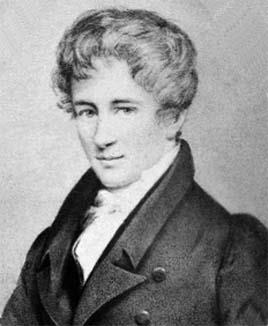
\includegraphics[width=0.85\textwidth]{../../images/python/page_008_img_01.jpeg}

\end{document}
